%
% File iscol2017.tex
%

\documentclass[11pt,a4paper]{article}
\usepackage{acl-onecolumn}
\usepackage{times}
\usepackage{url}
\usepackage{latexsym}
\usepackage{amsmath}
\usepackage{breqn}
\usepackage{pgfplotstable}
\usepackage{algorithm2e}
\usepackage{hhline}
\usepackage{multirow}
\usepackage[font=small]{caption}
\usepackage{subcaption}
\usepackage{color}
\usepackage{float}
\usepackage{lipsum,adjustbox}
\usepackage{tikz}
\usepackage{tikz-dependency}
\usepackage{enumitem}
\usepackage{xr}
\externaldocument{acl2017_supp}
\usetikzlibrary{shapes,fit,calc,er,positioning,intersections,decorations.shapes,mindmap,trees}
\tikzset{decorate sep/.style 2 args={decorate,decoration={shape backgrounds,shape=circle,
      shape size=#1,shape sep=#2}}}
\newcommand{\oa}[1]{\footnote{\color{red} #1}}
\newcommand{\daniel}[1]{\footnote{\color{blue} #1}}
\newcommand{\com}[1]{}
\newcommand{\parser}[1]{TUPA\textsubscript{#1}}
\newcommand{\secref}[1]{Section~\ref{#1}}
\newcommand{\figref}[1]{Figure~\ref{#1}}
\newcommand{\tabref}[1]{Table~\ref{#1}}
\DeclareMathOperator*{\argmin}{argmin}
\DeclareMathOperator*{\argmax}{argmax}
\SetKwRepeat{Do}{do}{while}

\hyphenation{SemEval}
\hyphenation{PARSEVAL}
\hyphenation{DAGParser}
\hyphenation{TurboSemanticParser}
\hyphenation{MaltParser}

\def\linkspace#1#2{\leavevmode
\def\tmp##1{\nolinebreak[2]\href{#1}{\hbox{##1}}}%
\xlinkspace#2 \relax}

\def\xlinkspace#1 #2{%
 \ifx\relax#2%
 \xlinkdash#1-\relax
 \else
 \xlinkdash#1 -\relax
 \expandafter\xlinkspace\expandafter#2%
 \fi}

\def\xlinkdash#1-#2{%
 \ifx\relax#2%
 \tmp{#1}%
 \else
 \tmp{#1-}%
 \expandafter\xlinkdash\expandafter#2%
 \fi}

\title{A Transition-Based Directed Acyclic Graph Parser for UCCA}

\author{Daniel Hershcovich$^{1,2}$ \\
  \\\And
  Omri Abend$^2$ \\
  $^1$The Edmond and Lily Safra Center for Brain Sciences \\
  $^2$School of Computer Science and Engineering \\
  Hebrew University of Jerusalem \\
  \texttt{\{danielh,oabend,arir\}@cs.huji.ac.il}
  \\\And
  Ari Rappoport$^2$
}

\date{}

\begin{document}
\maketitle

%%%%%%%%%%%%%%%%%%%%%%%%%%%%%%%%%%%%%%%%%%%%%%%%%%%%%%%%%%%%%%%
%%%%%%%%%%%%%%%%%     Abstract     %%%%%%%%%%%%%%%%%%%%%%%%%%%%
%%%%%%%%%%%%%%%%%%%%%%%%%%%%%%%%%%%%%%%%%%%%%%%%%%%%%%%%%%%%%%%
\begin{abstract}
  We present the first parser for UCCA, a
  cross-linguistically applicable framework for semantic
  representation, which builds on extensive
  typological work and supports rapid annotation.
  UCCA poses a challenge for existing parsing techniques,
  as it exhibits reentrancy (resulting in DAG structures),
  discontinuous structures and non-terminal nodes corresponding
  to complex semantic units. To our knowledge, the conjunction
  of these formal properties is not supported by any existing parser.
  Our transition-based parser, which uses a novel transition set
  and features based on bidirectional LSTMs,
  has value not just for UCCA parsing:
  its ability to handle more general graph structures can inform
  the development of parsers for other semantic DAG structures, 
  and in languages that frequently use discontinuous structures.
\end{abstract}


%%%%%%%%%%%%%%%%%%%%%%%%%%%%%%%%%%%%%%%%%%%%%%%%%%%%%%%%%%%%%%%
\section{Introduction}\label{sec:introduction}

Universal Conceptual Cognitive Annotation \cite[UCCA,][]{abend2013universal},
is a cross-linguistic and intuitive framework for semantic representation.

UCCA generates labeled DAGs whose leaves correspond to text tokens.
\figref{fig:examples} presents examples.

\begin{figure}[h]
  \begin{subfigure}{.35\textwidth}
  \scalebox{.7}{
  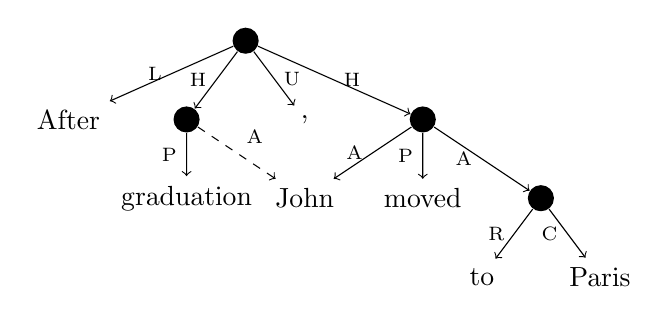
\begin{tikzpicture}[level distance=10mm, ->,
      every circle node/.append style={fill=black}]
    \node (ROOT) [circle] {}
      child {node (After) {After} edge from parent node[left] {\scriptsize L}}
      child {node (graduation) [circle] {}
      {
        child {node {graduation} edge from parent node[left] {\scriptsize P}}
      } edge from parent node[left] {\scriptsize H} }
      child {node {,} edge from parent node[right] {\scriptsize U}}
      child {node (moved) [circle] {}
      {
        child {node (John) {John} edge from parent node[left] {\scriptsize A}}
        child {node {moved} edge from parent node[left] {\scriptsize P}}
        child {node [circle] {}
        {
          child {node {to} edge from parent node[left] {\scriptsize R}}
          child {node {Paris} edge from parent node[left] {\scriptsize C}}
        } edge from parent node[left] {\scriptsize A} }
      } edge from parent node[right] {\scriptsize H} }
      ;
    \draw[dashed,->] (graduation) to node [auto] {\scriptsize A} (John);
  \end{tikzpicture}
  }
  \caption{}\label{fig:graduation}
  \end{subfigure}
  \begin{subfigure}{.18\textwidth}
  \scalebox{.7}{
  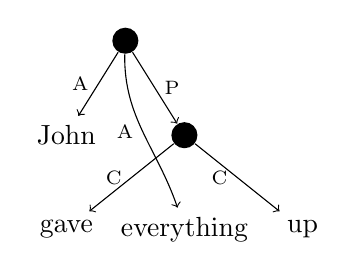
\begin{tikzpicture}[level distance=12mm, ->,
      every node/.append style={midway},
      every circle node/.append style={fill=black}]
    \node (ROOT) [circle] {}
      child {node {John} edge from parent node[left] {\scriptsize A}}
      child {node [circle] {}
      {
      	child {node {gave} edge from parent node[left] {\scriptsize C}}
      	child {node (everything) {everything} edge from parent[white]}
      	child {node {up} edge from parent node[left] {\scriptsize C}}
      } edge from parent node[right] {\scriptsize P} }
      ;
    \draw[bend right,->] (ROOT) to[out=-20, in=180] node [left] {\scriptsize A} (everything);
  \end{tikzpicture}
  }
  \caption{}\label{fig:gave}
  \end{subfigure}
  \begin{subfigure}{.3\textwidth}
  \scalebox{.7}{
  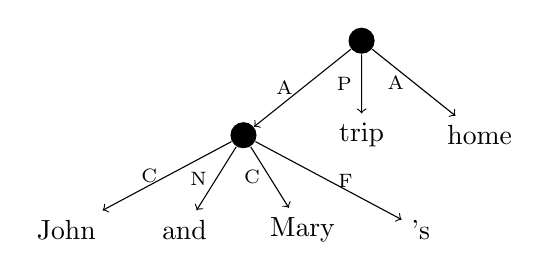
\begin{tikzpicture}[level distance=12mm, ->,
      every node/.append style={midway},
      every circle node/.append style={fill=black}]
    \node (ROOT) [circle] {}
      child {node [circle] {}
      {
        child {node {John} edge from parent node[left] {\scriptsize C}}
        child {node {and} edge from parent node[left] {\scriptsize N}}
        child {node {Mary} edge from parent node[left] {\scriptsize C}}
        child {node {'s} edge from parent node[right] {\scriptsize F}}
      } edge from parent node[left] {\scriptsize A} }
      child {node {trip} edge from parent node[left] {\scriptsize P}}
      child {node {home} edge from parent node[left] {\scriptsize A}}
      ;
  \end{tikzpicture}
  }
  \caption{}\label{fig:home}
  \end{subfigure}
  \begin{subfigure}{.15\textwidth}
  \begin{adjustbox}{width=.8\textwidth,margin=1pt,frame}
  \begin{tabular}{ll}
	  P & process \\
	  A & participant \\
	  H & linked scene \\
	  C & center \\
	  R & relator \\
	  N & connector \\
	  L & scene linker \\
	  U & punctuation \\
	  F & function unit
  \end{tabular}
  \end{adjustbox}
  \end{subfigure}
  \caption{\label{fig:examples}
    UCCA structures demonstrating three structural properties exhibited by
    the scheme.
  }
\end{figure}

While parsing technology
is well-established for syntactic parsing, UCCA
has several distinct properties
that distinguish it.
One such property is \textit{reentrancy},
namely sharing semantic units between predicates.
For instance, in \figref{fig:graduation},
``John'' is an argument of both ``graduation''
and ``moved'', yielding a DAG rather than a tree.
A second property is \textit{discontinuity},
as in \figref{fig:gave}, where ``gave up'' forms a discontinuous semantic unit.
Finally, UCCA uses \textit{non-terminal nodes}
to represent units comprising more than one word.
The use of non-terminal nodes is motivated by constructions with no clear head, including
coordination structures (e.g., ``John and Mary'' in \figref{fig:home})
and some multi-word expressions.
To our knowledge, no existing parser supports all structural properties required for UCCA
parsing.



%%%%%%%%%%%%%%%%%%%%%%%%%%%%%%%%%%%%%%%%%%%%%%%%%%%%%%%%%%%%%%%
\section{Transition-based UCCA Parsing}\label{sec:parser}


We present \parser{} (Transition-based UCCA Parser), the first UCCA parser, and
the first parser supporting the structural properties mentioned above.
We evaluate it on UCCA corpora, including out-of-domain.\footnote{All
parsing and conversion code is available at \url{https://github.com/danielhers/tupa}.}

\paragraph{Transition Set.}
In addition to the standard transitions in shift-reduce parsing, 
we include transitions for creating non-terminal nodes,
for creating primary and remote edges,
and for discontinuous parsing \cite{maier2015discontinuous}.
As in other work on
transition-based DAG dependency parsing \cite{sagae2008shift},
node and edge transitions do not pop the stack,
to support multiple parents.

\paragraph{Classifiers.}
We experiment with three classifiers, all used for greedy parsing:
structured perceptron with sparse features, \textbf{\parser{Sparse}};
feedforward neural network with dense embedding features, \textbf{\parser{MLP}};
and bidirectional LSTM with embedding features and a feedforward network
\textbf{\parser{BiLSTM}}.

%%%%%%%%%%%%%%%%%%%%%%%%%%%%%%%%%%%%%%%%%%%%%%%%%%%%%%%%%%%%%%%
\section{Experiments}\label{sec:exp_setup}

\paragraph{Data.}
Our experiments are on the UCCA Wikipedia corpus,
and the English part of the UCCA \textit{Twenty Thousand Leagues Under the Sea}
English-French parallel corpus as
out-of-domain data.\footnote{\mbox{\url{http://cs.huji.ac.il/~oabend/ucca.html}}}

\begin{table*}
	\begin{tabular}{l|ccc|ccc||ccc|ccc}
		& \multicolumn{6}{c||}{Wiki (in-domain)} & \multicolumn{6}{c}{20K Leagues (out-of-domain)} \\
		& \multicolumn{3}{c|}{Primary} & \multicolumn{3}{c||}{Remote}
		& \multicolumn{3}{c|}{Primary} & \multicolumn{3}{c}{Remote} \\
		& \textbf{LP} & \textbf{LR} & \textbf{LF} & \textbf{LP} & \textbf{LR} & \textbf{LF}
		& \textbf{LP} & \textbf{LR} & \textbf{LF} & \textbf{LP} & \textbf{LR} & \textbf{LF} \\
		\hline
		\parser{Sparse}
		& 64.5 & 63.7 & 64.1 & 19.8 & 13.4 & 16
		& 59.6 & 59.9 & 59.8 & 22.2 & 7.7 & 11.5 \\
		%\parser{Dense} 
		%& 59.1 & 58.9 & 59 & 17.4 & 12.4 & 14.5
		%& 57.0 & 57.9 & 57.4 & 10.8 & 4.2 & 6.0 \\
		\parser{MLP}
		& 65.2 & 64.6 & 64.9 & 23.7 & 13.2 & 16.9
		& 62.3 & 62.6 & 62.5 & 20.9 & 6.3 & 9.7 \\
		\parser{BiLSTM}
		& 74.4 & 72.7 & \textbf{73.5} & 47.4 & 51.6 & \textbf{49.4}
		& 68.7 & 68.5 & \textbf{68.6} & 38.6 & 18.8 & \textbf{25.3} \\
		\hline
		\multicolumn{8}{l}{\rule{0pt}{2ex} \footnotesize
		Bilexical Approximation (Dependency DAG Parsers)} \\
		\small Upper Bound
		%& \small 94.5 & \small 87.7 & \small 91 & \small 77.3 & \small 46.8 & \small 58.3
		%& \small 94.8 & \small 88 & \small 91.3 & \small 66.3 & \small 32.3 & \small 43.4 \\
		& & & \small 91 & & & \small 58.3
		& & & \small 91.3 & & & \small 43.4 \\
		DAGParser
		& 61.8 & 55.8 & 58.6 & 9.5 & 0.5 & 1
		& 56.4 & 50.6 & 53.4 & -- & 0 & 0 \\
		TurboParser
		& 57.7 & 46 & 51.2 & 77.8 & 1.8 & 3.7
		& 50.3 & 37.7 & 43.1 & 100 & 0.4 & 0.8 \\
		\hline
		\multicolumn{8}{l}{\rule{0pt}{2ex} \footnotesize
		Tree Approximation (Constituency Tree Parser)} \\
		\small Upper Bound
		%& \small 100 & \small 100 & \small 100 & & &
		%& \small 100 & \small 100 & \small 100 \\
		& & & \small 100 & & & \small --
		& & & \small 100 & & & \small -- \\
		\textsc{uparse}
		& 60.9 & 61.2 & 61.1 & -- & -- & --
		& 52.7 & 52.8 & 52.8 & -- & -- & -- \\
		\hline
		\multicolumn{8}{l}{\rule{0pt}{2ex} \footnotesize
		Bilexical Tree Approximation (Dependency Tree Parsers)} \\
		\small Upper Bound
		%& \small 94.5 & \small 87.7 & \small 91 & & &
		%& \small 94.8 & \small 88 & \small 91.3 \\
		& & & \small 91 & & & \small --
		& & & \small 91.3 & & & \small -- \\
		MaltParser
		& 62.8 & 57.7 & 60.2 & -- & -- & --
		& 57.8 & 53 & 55.3 & -- & -- & -- \\
		LSTM Parser
		& 73.2 & 66.9 & 69.9 & -- & -- & --
		& 66.1 & 61.1 & 63.5 & -- & -- & --
	\end{tabular}
	\caption{
	  Experimental results, in percents, on the \textit{Wiki} test set (left)
	  and the \textit{20K Leagues} set (right).
	}
	\label{table:results}
\end{table*}

\paragraph{Comparison to bilexical graph and tree parsers.}
As no direct comparison with existing parsers is possible,
we compare \parser{} to existing parsers
by converting UCCA to formats they support,
training them, and evaluating the result after converting back.

\paragraph{Results}

\tabref{table:results} presents our main experimental results
\parser{BiLSTM} obtains substantially higher scores than \parser{MLP}
and all other parsers, on both primary and remote edges,
both in the in-domain and out-of-domain settings.
Its performance in absolute terms, of 73.5\% F-score on primary edges,
is encouraging in light of
UCCA's inter-annotator agreement of 80--85\%
F-score on them \cite{abend2013universal}.


\bibliography{references}
\bibliographystyle{acl_natbib}

\end{document}
